\section{Overview}
In this chapter, we initiate a comprehensive analysis by systematically comparing each statistical measure derived from our simulations. We focus on evaluating the mean values, covariance matrices, and correlation matrices obtained from the \emph{BIGBOX} and \emph{TILED} simulations to assess their consistency and understand the underlying discrepancies.

Figures~\ref{fig:cl_main} through \ref{fig:mfs_cov} provide detailed visualizations of the mean values, variances, covariance matrices, and correlation matrices for each statistical measure under consideration. For each statistic, one figure illustrates the comparison of mean values and variances, while another figure presents the comparison of covariance and correlation matrices. Due to limitations in space, we have included only the covariance matrix comparisons for the bispectrum and Minkowski Functionals.

From these figures, we observe that the mean values of most statistical measures exhibit excellent agreement between the BIGBOX and TILED simulations, with differences remaining below $1\%$ across the majority of the studied range. However, notable deviations occur at low $\nu$ values for peak counts, minima, and the Minkowski Functionals $V_1$ and $V_2$. These deviations are attributed to the limited resolution of the simulations, which affects the accurate detection of regions with the lowest density contrasts.

Analyzing the covariance matrices reveals that, except for the bispectrum, the ratios of covariance matrix elements between the BIGBOX and TILED simulations are consistently greater than unity. This indicates that the BIGBOX simulations yield higher covariance values compared to the TILED simulations, and this discrepancy becomes more pronounced at higher source redshifts. The bispectrum, on the other hand, exhibits noisy covariance matrices without a clear trend, making it challenging to draw definitive conclusions for this statistic.

Examining the correlation matrices further, we focus on the off-diagonal elements to assess the degree of inter-bin correlations. For statistical measures that are not inherently correlated, the off-diagonal elements remain close to unity, as expected. In contrast, the power spectrum shows off-diagonal elements that exceed unity, displaying a clear increasing trend with higher source redshifts. This behavior aligns with theoretical predictions of super-sample covariance effects, as detailed in \citet{PhysRevD.87.123504}, suggesting that larger-scale modes beyond the survey volume contribute to the observed correlations.

Overall, these findings support the hypothesis that super-sample covariance significantly impacts the statistical measures derived from our simulations. The discrepancies observed between the BIGBOX and TILED simulations emphasize the importance of considering super-sample effects in cosmological analyses. We will explore these effects in greater depth and seek further validation in the subsequent discussion chapter.

\begin{figure}[p]
    \centering
    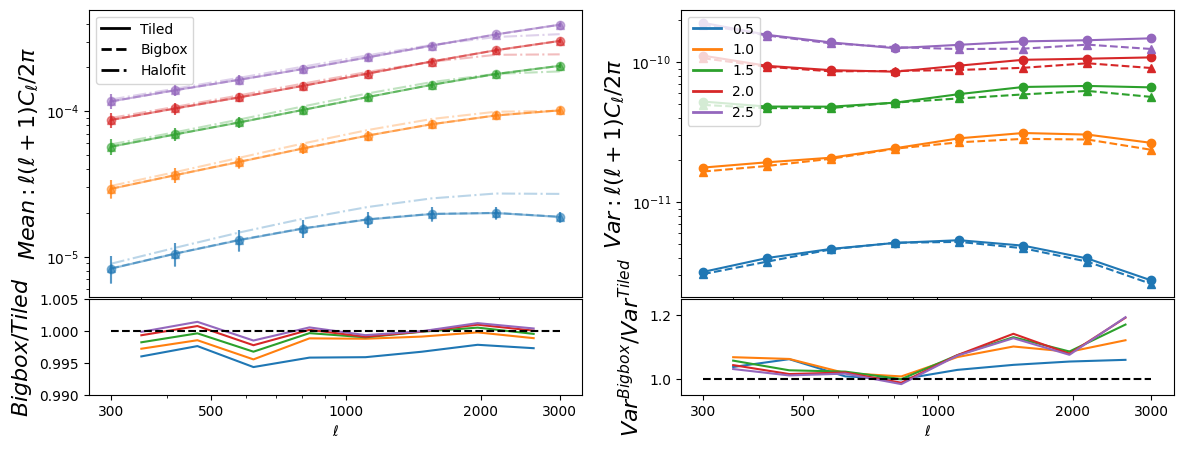
\includegraphics[width=\textwidth]{figures/results/cl_main.png}
    \caption{Comparison of the mean values of the angular power spectrum ($C^{\kappa\kappa}_{\ell}$) for different source redshifts ($z_s = 0.5, 1.0, 1.5, 2.0, 2.5$) obtained from the BIGBOX (solid lines) and TILED (dashed lines) simulations. The lower subplots show the ratio of the TILED to BIGBOX mean values, with a reference line at unity to facilitate the assessment of agreement between the two simulations.}
    \label{fig:cl_main}
    \vspace{2cm}
    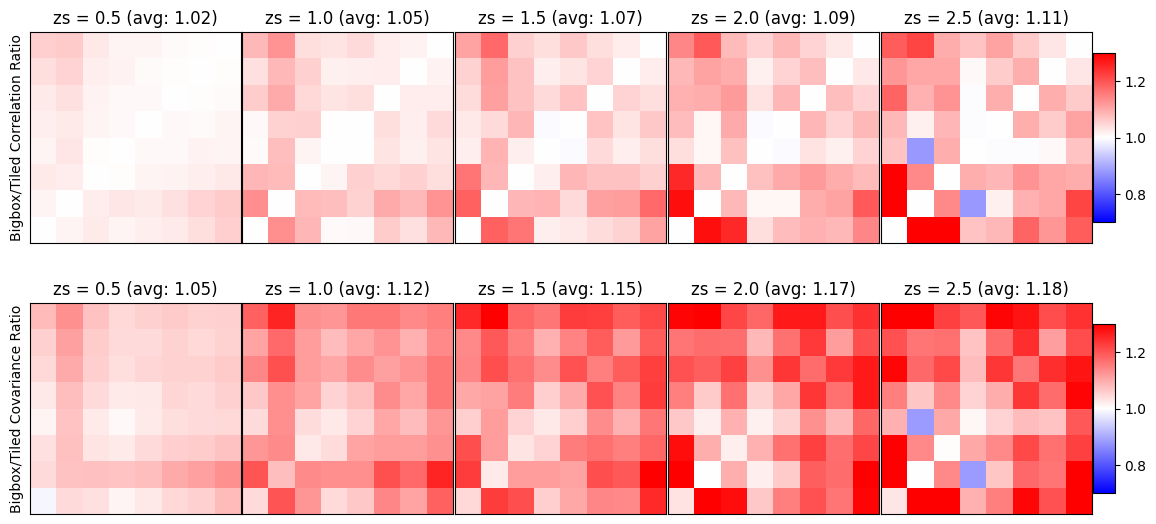
\includegraphics[width=\textwidth]{figures/results/cl_cov.png}
    \caption{Comparison of the covariance matrices and correlation matrices of the angular power spectrum ($C^{\kappa\kappa}_{\ell}$) between the BIGBOX and TILED simulations for various source redshifts ($z_s = 0.5, 1.0, 1.5, 2.0, 2.5$). The displayed ratios represent the element-wise division of the covariance and correlation matrices from the TILED simulations by those from the BIGBOX simulations. The "avg" denotes the average ratio of the considered matrix elements.}
    \label{fig:cl_cov}
\end{figure}

\begin{figure}[p]
    \centering
    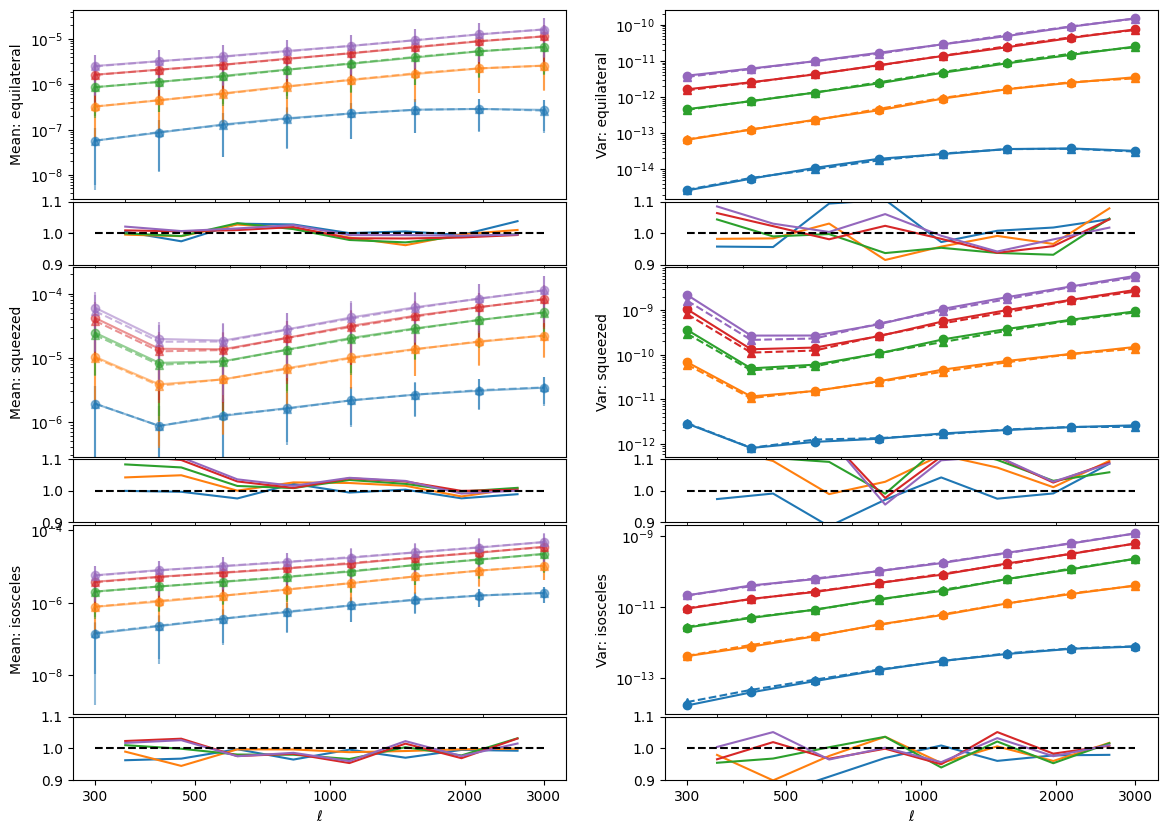
\includegraphics[width=\textwidth]{figures/results/bl_main.png}
    \caption{Same as Figure~\ref{fig:cl_main}, but for the bispectrum. }
    \label{fig:bl_main}
    \vspace{0.5cm}
    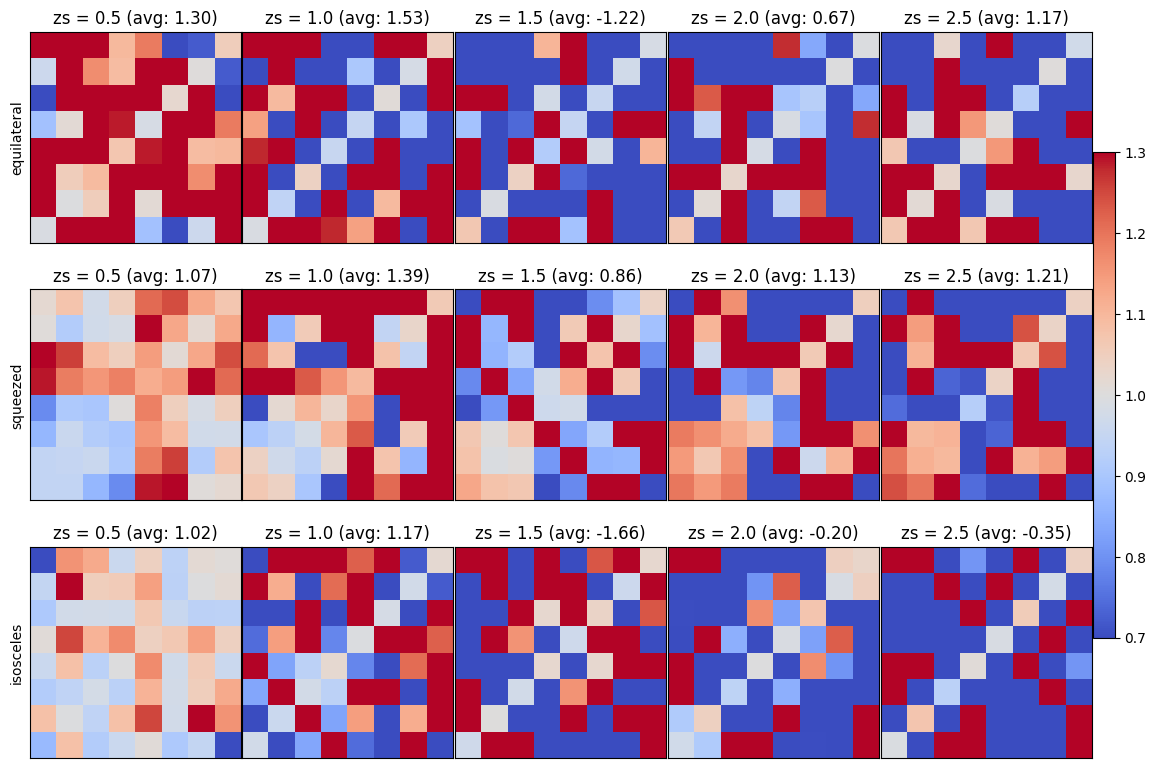
\includegraphics[width=\textwidth]{figures/results/bl_cov.png}
    \caption{Similar to Figure~\ref{fig:cl_cov}, but for the covariance matrices of the bispectrum. The noisy nature of the bispectrum covariance makes it challenging to discern clear trends between the simulations.}
    \label{fig:bl_cov}
\end{figure}

\begin{figure}[p]
    \centering
    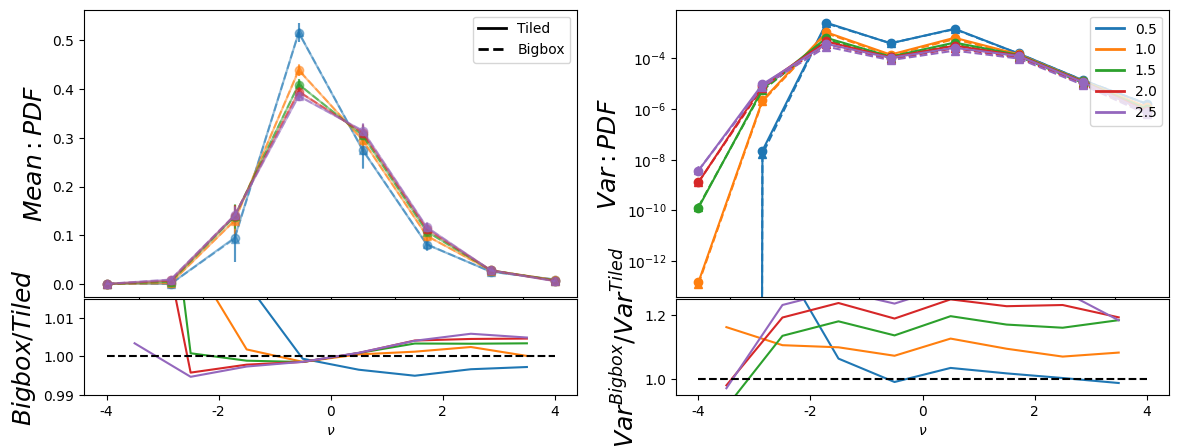
\includegraphics[width=\textwidth]{figures/results/pdf_main.png}
    \caption{Same as Figure~\ref{fig:cl_main}, but for the probability density function (PDF) of the convergence field. The comparison highlights the agreement in mean PDF values between the simulations across different redshifts.}
    \label{fig:pdf_main}
    \vspace{2cm}
    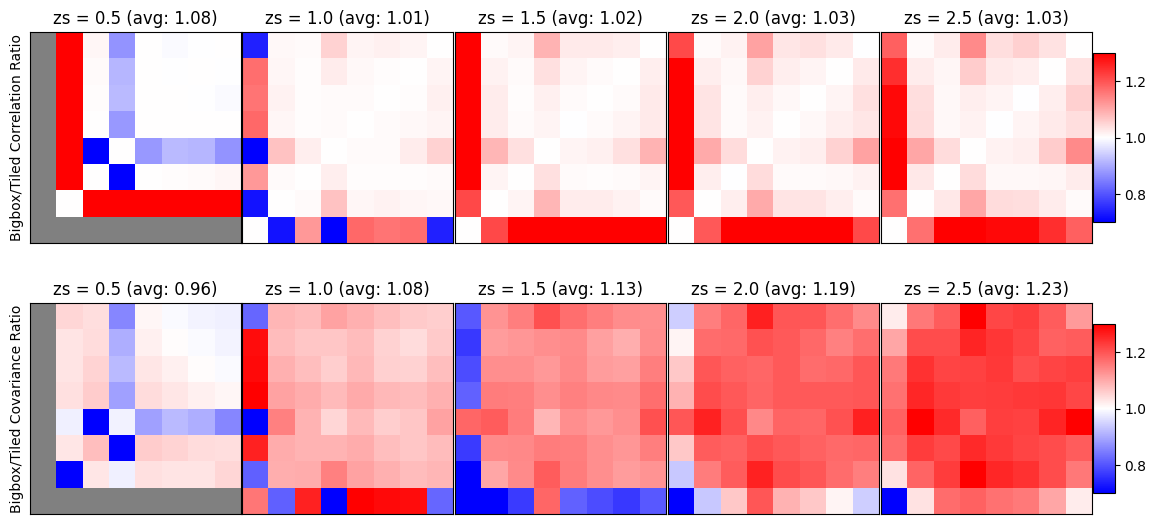
\includegraphics[width=\textwidth]{figures/results/pdf_cov.png}
    \caption{Same as Figure~\ref{fig:cl_cov}, but for the covariance matrices of the PDF. The covariance ratios indicate higher covariance in the BIGBOX simulations, particularly at higher redshifts.}
    \label{fig:pdf_cov}
\end{figure}

\begin{figure}[p]
    \centering
    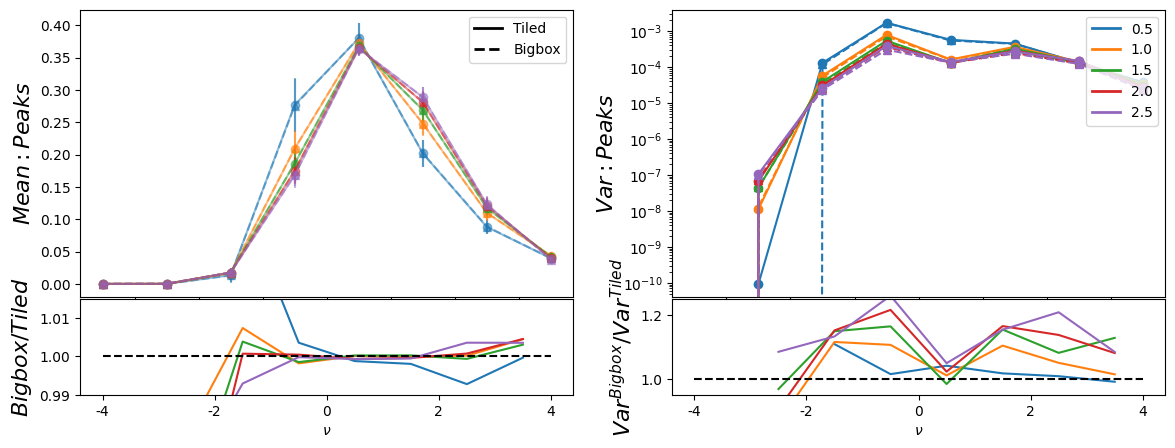
\includegraphics[width=\textwidth]{figures/results/peaks_main.png}
    \caption{Same as Figure~\ref{fig:cl_main}, but for peak counts in the convergence maps. The analysis reveals deviations at low $\nu$ values due to resolution limitations affecting low-density regions.}
    \label{fig:peak_main}
    \vspace{2cm}
    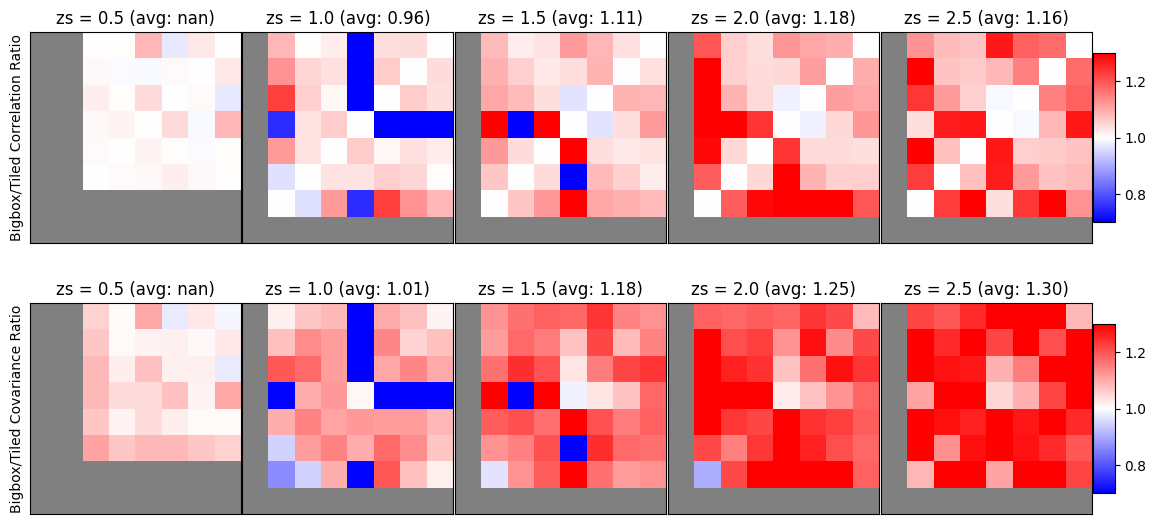
\includegraphics[width=\textwidth]{figures/results/peaks_cov.png}
    \caption{Same as Figure~\ref{fig:cl_cov}, but for the covariance matrices of peak counts. The covariance ratios suggest increased covariance in the BIGBOX simulations, with pronounced effects at higher redshifts.}
    \label{fig:peak_cov}
\end{figure}

\begin{figure}[p]
    \centering
    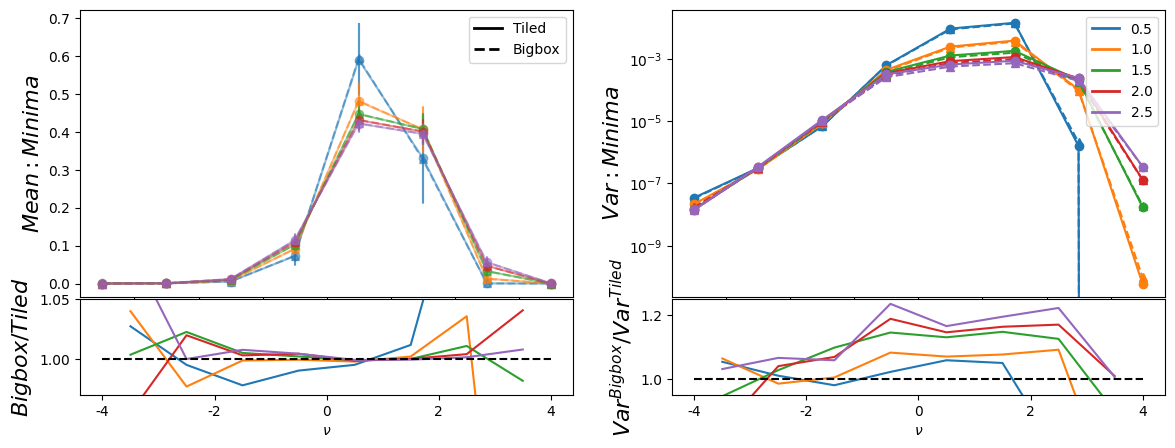
\includegraphics[width=\textwidth]{figures/results/minima_main.png}
    \caption{Same as Figure~\ref{fig:cl_main}, but for minima in the convergence maps. The comparison underscores the simulation's limitations at resolving low-density minima accurately.}
    \label{fig:min_main}
    \vspace{2cm}
    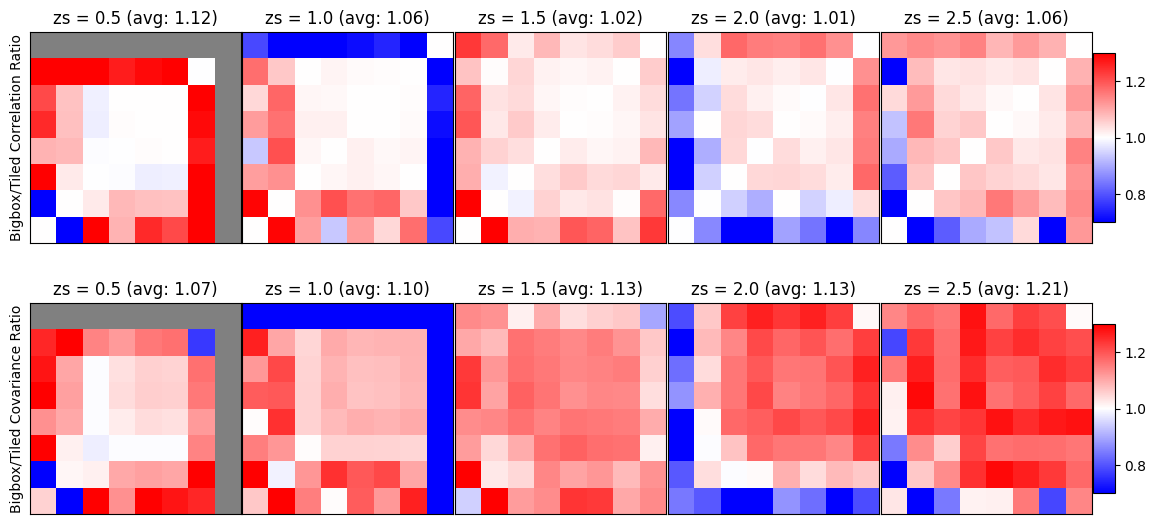
\includegraphics[width=\textwidth]{figures/results/minima_cov.png}
    \caption{Same as Figure~\ref{fig:cl_cov}, but for the covariance matrices of minima. The covariance ratios reflect higher values in the BIGBOX simulations, consistent with other statistical measures.}
    \label{fig:min_cov}
\end{figure}

\begin{figure}[p]
    \centering
    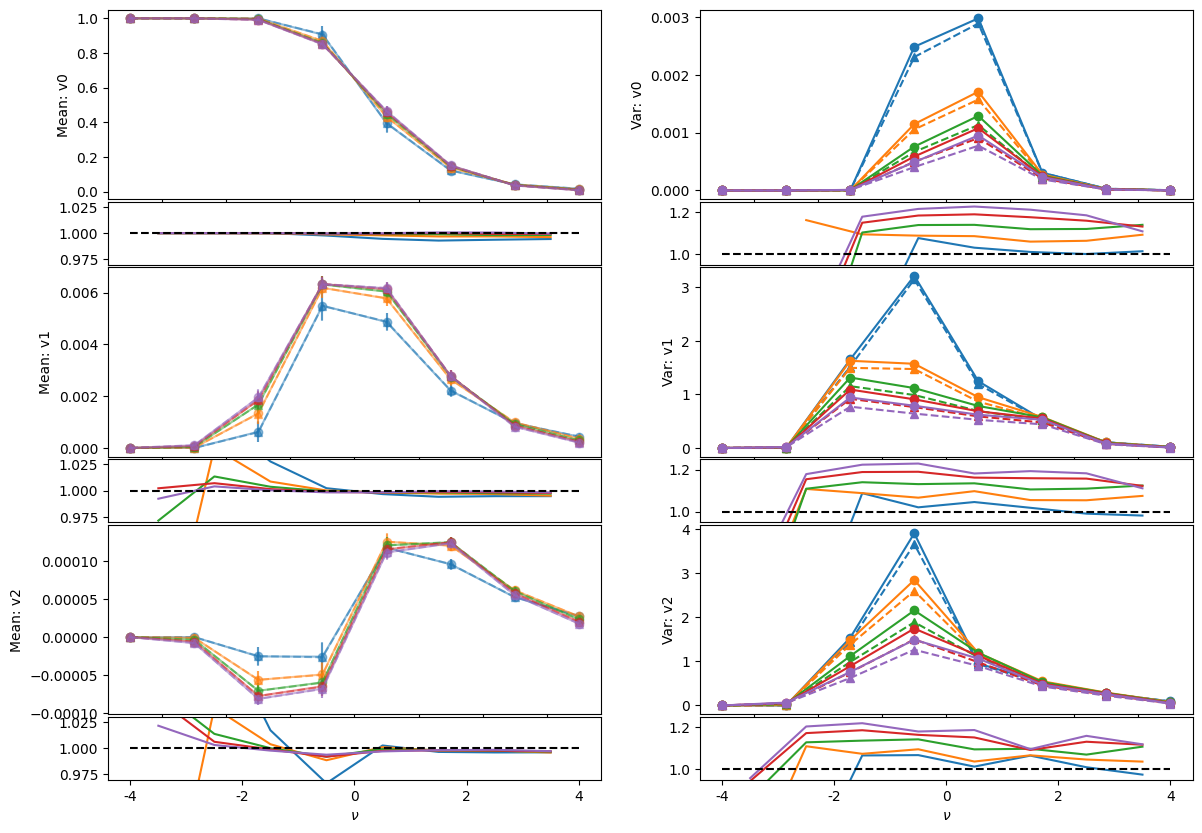
\includegraphics[width=\textwidth]{figures/results/mfs_main.png}
    \caption{Same as Figure~\ref{fig:cl_main}, but for Minkowski Functionals (area $V_0$, perimeter $V_1$, and genus $V_2$). The agreement in mean values between simulations is generally good, with some discrepancies at extreme density thresholds.}
    \label{fig:mfs_main}
    \vspace{0.5cm}
    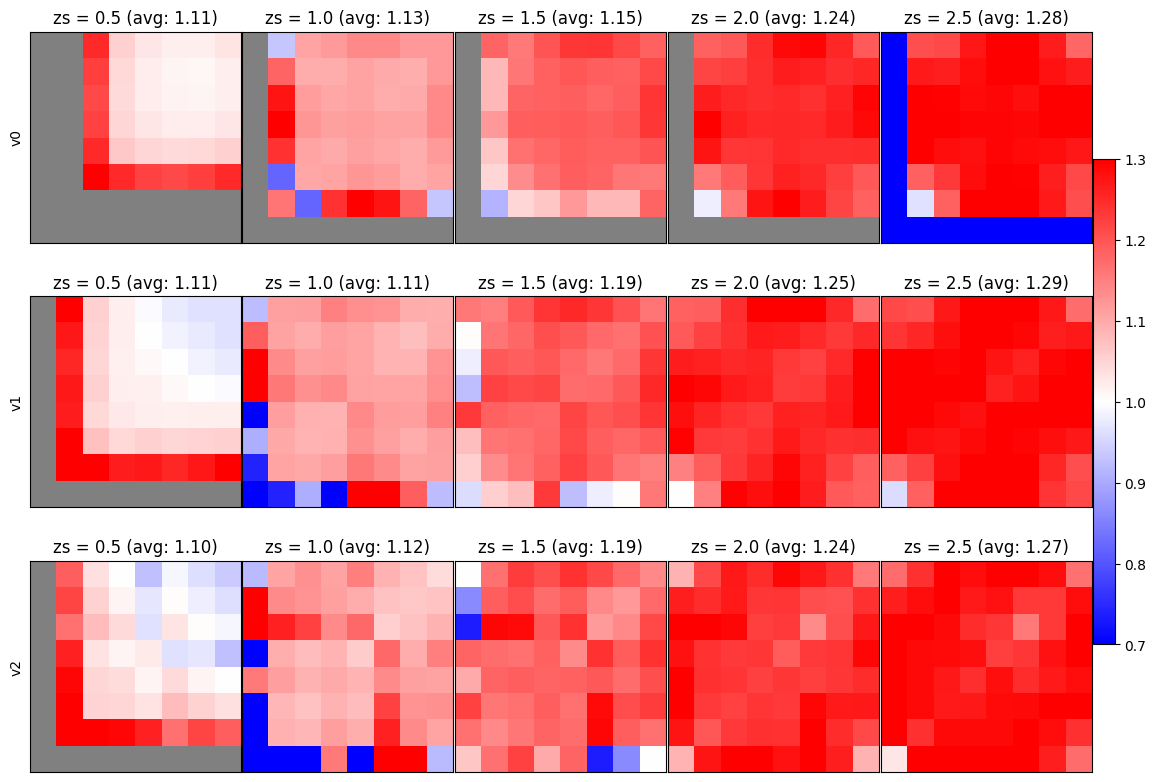
\includegraphics[width=\textwidth]{figures/results/mfs_cov.png}
    \caption{Similar to Figure~\ref{fig:cl_cov}, but for the covariance matrices of Minkowski Functionals. }
    \label{fig:mfs_cov}
\end{figure}

\section{Effects of Noise}
To assess the impact of observational noise, we have introduced five different shape noise levels into the simulations. Due to the significant influence of noise on higher-order statistics, the bispectrum has been excluded from this part of the analysis.

Figures~\ref{fig:avg_noise_cov} and \ref{fig:avg_noise_corr} illustrate how the average ratios of covariance matrices and correlation matrices change with varying shape noise levels. Except for the angular power spectrum, the non-Correlation statistics exhibit stable covariance ratios across different noise levels. 

\begin{figure}
    \centering
    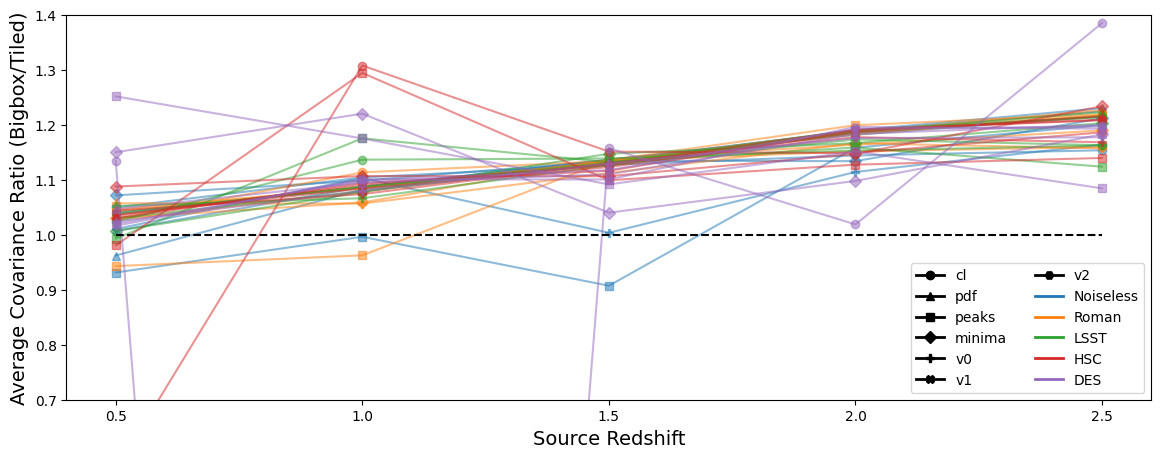
\includegraphics[width=0.6\textwidth]{figures/results/avg_cov_ratio_ngal.png}
    \caption{Average ratio of covariance matrices of statistical measures between the BIGBOX and TILED simulations for different shape noise levels (see Table~\ref{tab:noise}). The increasing trend indicates does not affected by the noise level.}
    \label{fig:avg_noise_cov}
    \vspace{0.5cm}
    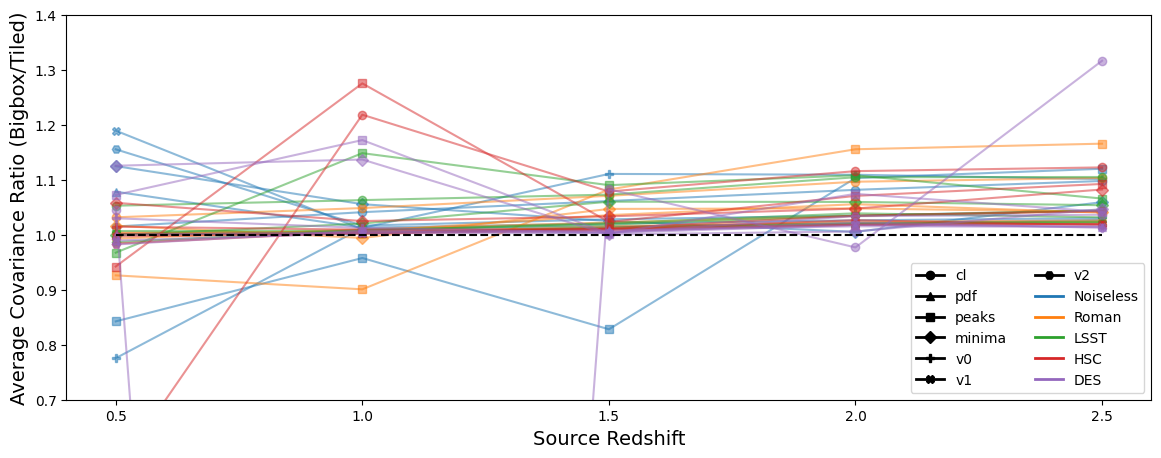
\includegraphics[width=0.6\textwidth]{figures/results/avg_corr_ratio_ngal.png}
    \caption{Same as Figure~\ref{fig:avg_noise_cov}, but for the correlation matrices. The off-diagonal elements compared to the diagonal elements do not show a clear trend with noise levels.}
    \label{fig:avg_noise_corr}
    \vspace{0.5cm}
    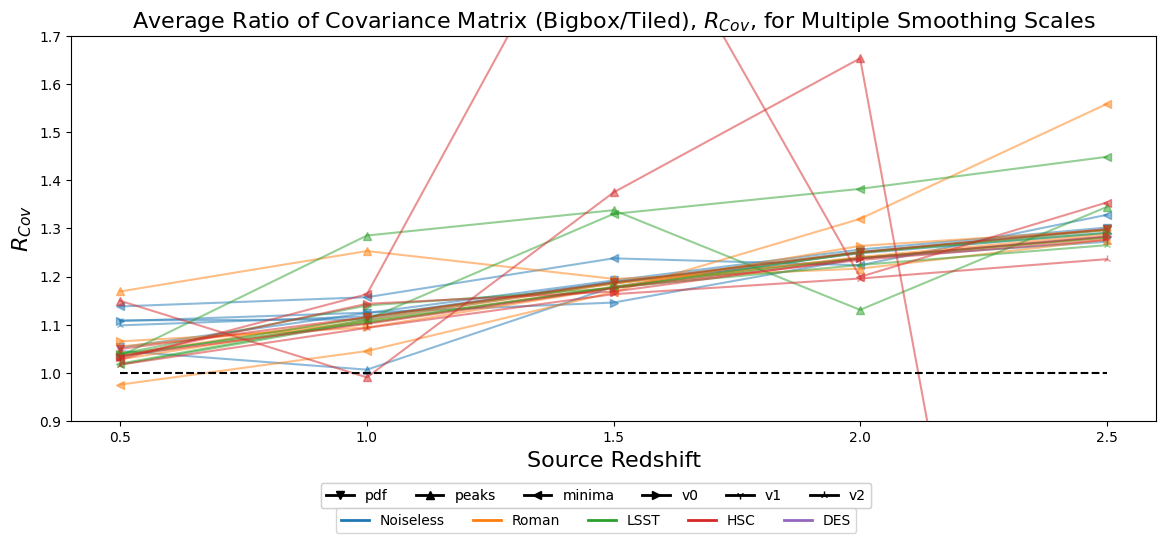
\includegraphics[width=0.6\textwidth]{figures/results/avg_cov_ratio_sl.png}
    \caption{Average ratio of covariance matrices of statistical measures between the BIGBOX and TILED simulations for different smoothing scales. Larger smoothing scales lead to increased discrepancies in covariance estimates due to the loss of small-scale information.}
    \label{fig:avg_sl_cov}
    \vspace{0.5cm}
    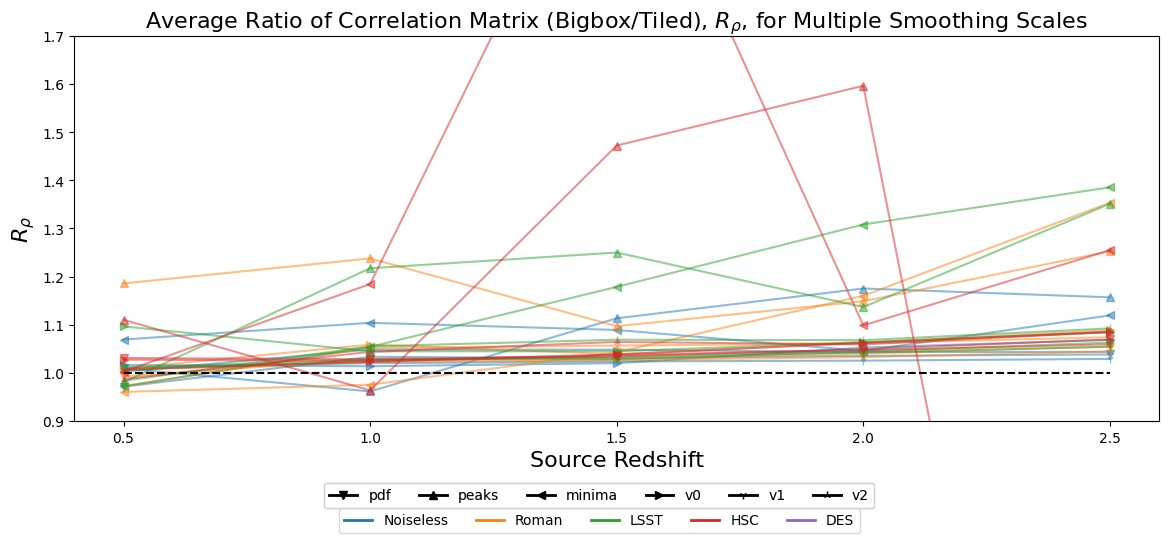
\includegraphics[width=0.6\textwidth]{figures/results/avg_corr_ratio_sl.png}
    \caption{Same as Figure~\ref{fig:avg_sl_cov}, but for the correlation matrices. The instability at larger smoothing scales reflects the challenges in capturing correlations at reduced resolutions.}
    \label{fig:avg_sl_corr}
\end{figure}

Figures~\ref{fig:cl_noise} and \ref{fig:ng_noise} demonstrate how the ratios of covariance matrices for the angular power spectrum and the non-correlation statistics change with different shape noise levels. The results indicate that the angular power spectrum and minima are particularly sensitive to the shape noise level, exhibiting significant variations in their covariance matrices. In contrast, other non-correlation statistics remain more robust against changes in the shape noise level, maintaining relatively stable off-diagonal elements in their covariance matrices.

\begin{figure}[p]
    \centering
    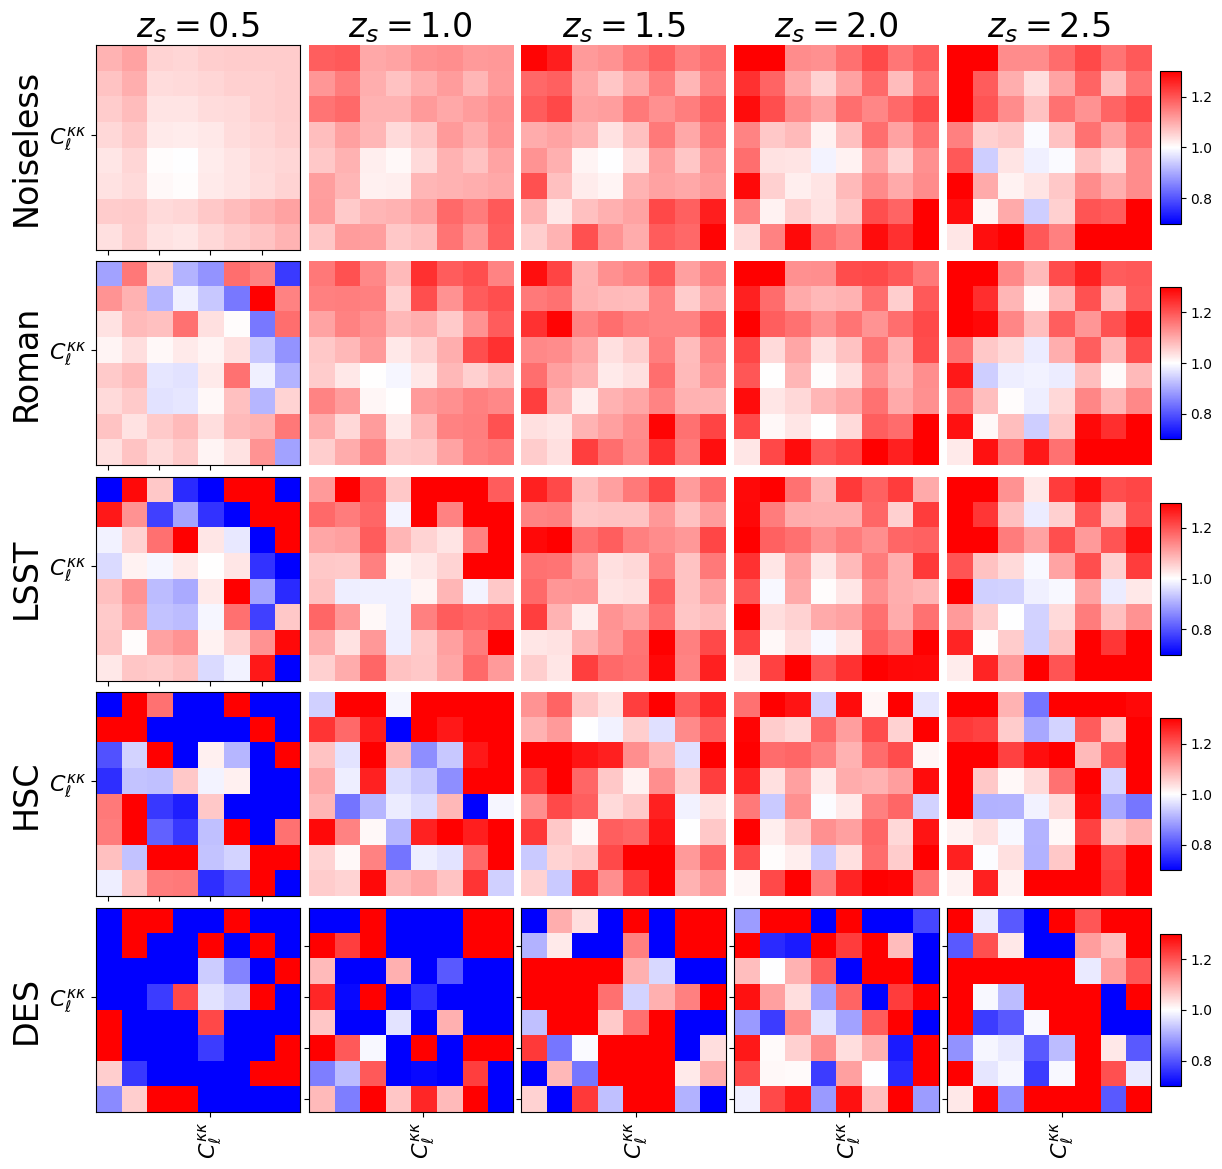
\includegraphics[width=0.6\textwidth]{figures/results/correlation_cov_noise.png}
    \caption{Ratio of covariance matrices of the angular power spectrum ($C^{\kappa\kappa}_{\ell}$) between the BIGBOX and TILED simulations for different shape noise levels (see Table~\ref{tab:noise}). The sensitivity of the power spectrum to noise is evident from the fluctuating covariance ratios with higher noise levels.}
    \label{fig:cl_noise}
    \vspace{0.5cm}
    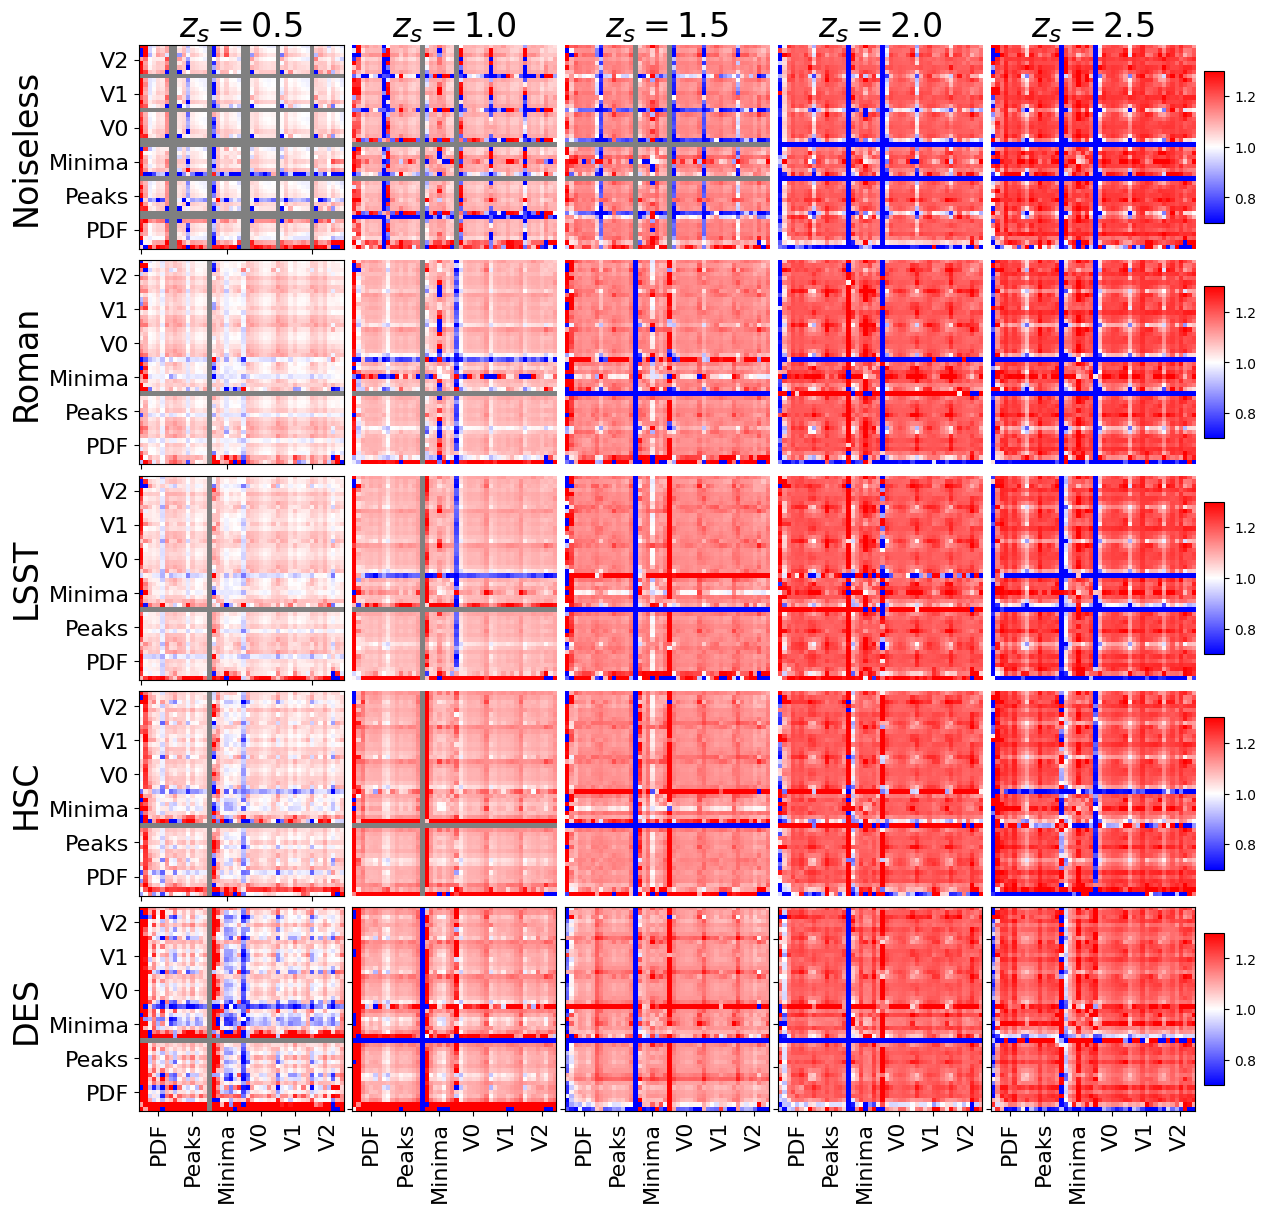
\includegraphics[width=0.8\textwidth]{figures/results/nongaussian_cov_noise.png}
    \caption{Same as Figure~\ref{fig:cl_noise}, but for the non-Gaussian statistical measures. The robustness of these measures against noise variations is reflected in the relatively stable covariance ratios.}
    \label{fig:ng_noise}
\end{figure}

\section{Effects of Smoothing Scale}
To evaluate the impact of smoothing on the statistical measures, we have applied four different smoothing scales to the simulations. Smoothing affects the resolution of the convergence maps and can influence the detection of small-scale structures.

Figures~\ref{fig:avg_sl_cov} and \ref{fig:avg_sl_corr} show how the average ratios of covariance matrices and correlation matrices change with varying smoothing scales. The ratios become more unstable due to the smoothing effect washing out small-scale structures.

Figure~\ref{fig:ng_smoothing} illustrates the effects of smoothing scale on non-Correlation statistical measures. As the smoothing scale increases, the finer structures in the convergence maps are blurred, leading to changes in the statistical properties. The blank bins that previously contained little or no signal begin to be filled due to the spread of signals from neighboring bins, while the overall signal intensity is redistributed.

\begin{figure}
    \centering
    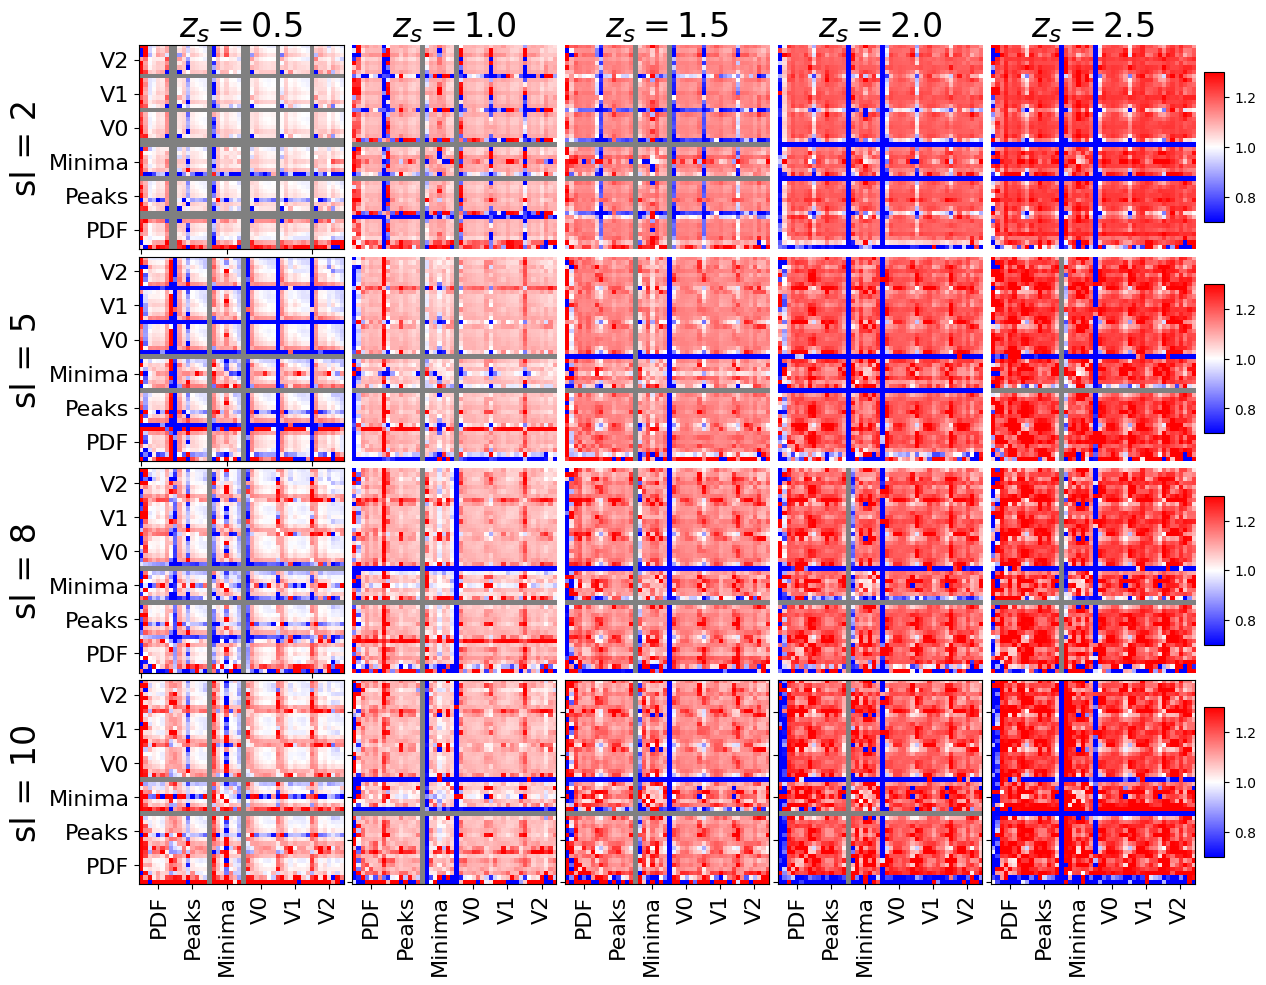
\includegraphics[width=0.8\textwidth]{figures/results/nongaussian_cov_sl.png}
    \caption{Same as Figure~\ref{fig:ng_noise}, but showing the impact of different smoothing scales on the covariance matrices of non-Gaussian statistical measures. The results emphasize how increased smoothing affects the detection and characterization of small-scale features.}
    \label{fig:ng_smoothing}
\end{figure}